\renewcommand{\slideid}{L3-PY06}
\begin{frame}[c]{Python lab 3: sweep the boundary penalty}
\small
Keep the 1D Poisson problem; replace $x(1-x)N_\theta(x)$ by $N_\theta(x)$.
\lstinputlisting[style=pythonlab]{experiments/snippets/boundary_loss.py}
\begin{block}{Change one setting at a time}
$\lambda_b\in\{0.01,0.1,1,10,100,1000\}$; identical initial weights,
collocation points, learning rate, and \BoundarySteps\ Adam updates.
The hard-constraint run gets the same update budget.
\end{block}
\labnote{The residual is divided by $\pi^2$, so the weight sweep refers to that
specific scaling. No L-BFGS refinement is used in this comparison.}
\end{frame}

\renewcommand{\slideid}{L3-PY07}
\begin{frame}[c]{Python output: boundary accuracy is only one diagnostic}
\small
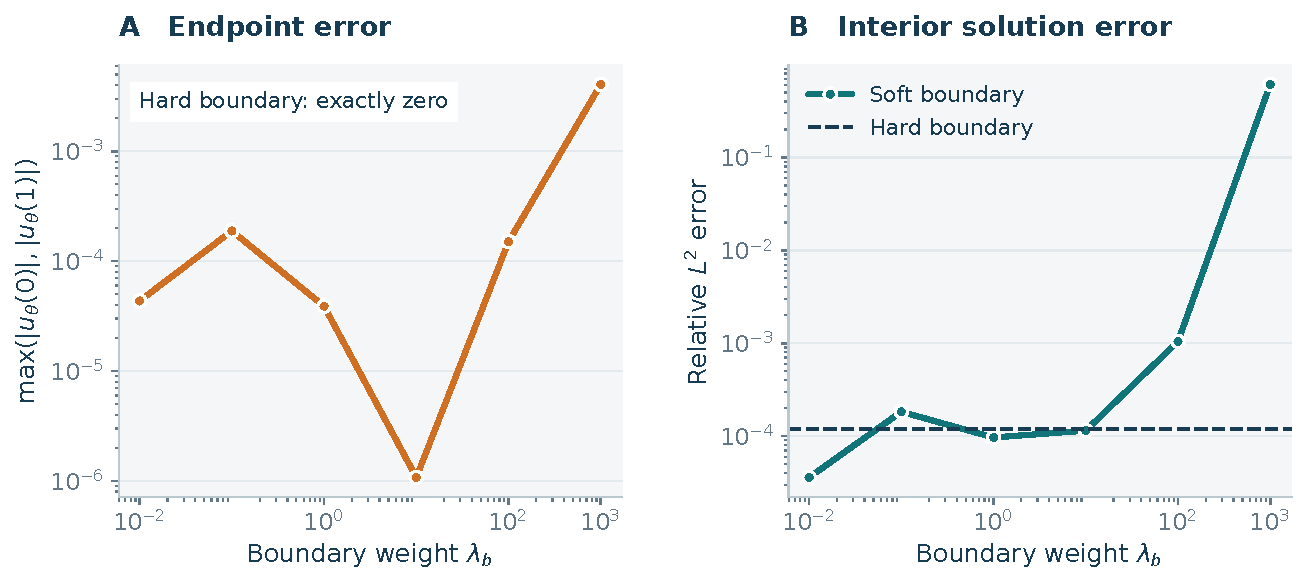
\includegraphics[width=\textwidth]{experiments/figures/boundary_sweep.pdf}
\begin{block}{Read both panels together}
Check the interior error as well as the boundary error.
The hard-constraint baseline has zero endpoint error exactly.
\end{block}
\labnote{These results use one seed and one training budget. Repeat the sweep
with other settings before choosing a penalty weight.}
\end{frame}
\renewcommand{\slideid}{L3}
